% Options for packages loaded elsewhere
\PassOptionsToPackage{unicode}{hyperref}
\PassOptionsToPackage{hyphens}{url}
\PassOptionsToPackage{dvipsnames,svgnames,x11names}{xcolor}
%
\documentclass[
  letterpaper,
  DIV=11,
  numbers=noendperiod]{scrartcl}

\usepackage{amsmath,amssymb}
\usepackage{iftex}
\ifPDFTeX
  \usepackage[T1]{fontenc}
  \usepackage[utf8]{inputenc}
  \usepackage{textcomp} % provide euro and other symbols
\else % if luatex or xetex
  \usepackage{unicode-math}
  \defaultfontfeatures{Scale=MatchLowercase}
  \defaultfontfeatures[\rmfamily]{Ligatures=TeX,Scale=1}
\fi
\usepackage{lmodern}
\ifPDFTeX\else  
    % xetex/luatex font selection
\fi
% Use upquote if available, for straight quotes in verbatim environments
\IfFileExists{upquote.sty}{\usepackage{upquote}}{}
\IfFileExists{microtype.sty}{% use microtype if available
  \usepackage[]{microtype}
  \UseMicrotypeSet[protrusion]{basicmath} % disable protrusion for tt fonts
}{}
\makeatletter
\@ifundefined{KOMAClassName}{% if non-KOMA class
  \IfFileExists{parskip.sty}{%
    \usepackage{parskip}
  }{% else
    \setlength{\parindent}{0pt}
    \setlength{\parskip}{6pt plus 2pt minus 1pt}}
}{% if KOMA class
  \KOMAoptions{parskip=half}}
\makeatother
\usepackage{xcolor}
\setlength{\emergencystretch}{3em} % prevent overfull lines
\setcounter{secnumdepth}{5}
% Make \paragraph and \subparagraph free-standing
\makeatletter
\ifx\paragraph\undefined\else
  \let\oldparagraph\paragraph
  \renewcommand{\paragraph}{
    \@ifstar
      \xxxParagraphStar
      \xxxParagraphNoStar
  }
  \newcommand{\xxxParagraphStar}[1]{\oldparagraph*{#1}\mbox{}}
  \newcommand{\xxxParagraphNoStar}[1]{\oldparagraph{#1}\mbox{}}
\fi
\ifx\subparagraph\undefined\else
  \let\oldsubparagraph\subparagraph
  \renewcommand{\subparagraph}{
    \@ifstar
      \xxxSubParagraphStar
      \xxxSubParagraphNoStar
  }
  \newcommand{\xxxSubParagraphStar}[1]{\oldsubparagraph*{#1}\mbox{}}
  \newcommand{\xxxSubParagraphNoStar}[1]{\oldsubparagraph{#1}\mbox{}}
\fi
\makeatother

\usepackage{color}
\usepackage{fancyvrb}
\newcommand{\VerbBar}{|}
\newcommand{\VERB}{\Verb[commandchars=\\\{\}]}
\DefineVerbatimEnvironment{Highlighting}{Verbatim}{commandchars=\\\{\}}
% Add ',fontsize=\small' for more characters per line
\usepackage{framed}
\definecolor{shadecolor}{RGB}{241,243,245}
\newenvironment{Shaded}{\begin{snugshade}}{\end{snugshade}}
\newcommand{\AlertTok}[1]{\textcolor[rgb]{0.68,0.00,0.00}{#1}}
\newcommand{\AnnotationTok}[1]{\textcolor[rgb]{0.37,0.37,0.37}{#1}}
\newcommand{\AttributeTok}[1]{\textcolor[rgb]{0.40,0.45,0.13}{#1}}
\newcommand{\BaseNTok}[1]{\textcolor[rgb]{0.68,0.00,0.00}{#1}}
\newcommand{\BuiltInTok}[1]{\textcolor[rgb]{0.00,0.23,0.31}{#1}}
\newcommand{\CharTok}[1]{\textcolor[rgb]{0.13,0.47,0.30}{#1}}
\newcommand{\CommentTok}[1]{\textcolor[rgb]{0.37,0.37,0.37}{#1}}
\newcommand{\CommentVarTok}[1]{\textcolor[rgb]{0.37,0.37,0.37}{\textit{#1}}}
\newcommand{\ConstantTok}[1]{\textcolor[rgb]{0.56,0.35,0.01}{#1}}
\newcommand{\ControlFlowTok}[1]{\textcolor[rgb]{0.00,0.23,0.31}{\textbf{#1}}}
\newcommand{\DataTypeTok}[1]{\textcolor[rgb]{0.68,0.00,0.00}{#1}}
\newcommand{\DecValTok}[1]{\textcolor[rgb]{0.68,0.00,0.00}{#1}}
\newcommand{\DocumentationTok}[1]{\textcolor[rgb]{0.37,0.37,0.37}{\textit{#1}}}
\newcommand{\ErrorTok}[1]{\textcolor[rgb]{0.68,0.00,0.00}{#1}}
\newcommand{\ExtensionTok}[1]{\textcolor[rgb]{0.00,0.23,0.31}{#1}}
\newcommand{\FloatTok}[1]{\textcolor[rgb]{0.68,0.00,0.00}{#1}}
\newcommand{\FunctionTok}[1]{\textcolor[rgb]{0.28,0.35,0.67}{#1}}
\newcommand{\ImportTok}[1]{\textcolor[rgb]{0.00,0.46,0.62}{#1}}
\newcommand{\InformationTok}[1]{\textcolor[rgb]{0.37,0.37,0.37}{#1}}
\newcommand{\KeywordTok}[1]{\textcolor[rgb]{0.00,0.23,0.31}{\textbf{#1}}}
\newcommand{\NormalTok}[1]{\textcolor[rgb]{0.00,0.23,0.31}{#1}}
\newcommand{\OperatorTok}[1]{\textcolor[rgb]{0.37,0.37,0.37}{#1}}
\newcommand{\OtherTok}[1]{\textcolor[rgb]{0.00,0.23,0.31}{#1}}
\newcommand{\PreprocessorTok}[1]{\textcolor[rgb]{0.68,0.00,0.00}{#1}}
\newcommand{\RegionMarkerTok}[1]{\textcolor[rgb]{0.00,0.23,0.31}{#1}}
\newcommand{\SpecialCharTok}[1]{\textcolor[rgb]{0.37,0.37,0.37}{#1}}
\newcommand{\SpecialStringTok}[1]{\textcolor[rgb]{0.13,0.47,0.30}{#1}}
\newcommand{\StringTok}[1]{\textcolor[rgb]{0.13,0.47,0.30}{#1}}
\newcommand{\VariableTok}[1]{\textcolor[rgb]{0.07,0.07,0.07}{#1}}
\newcommand{\VerbatimStringTok}[1]{\textcolor[rgb]{0.13,0.47,0.30}{#1}}
\newcommand{\WarningTok}[1]{\textcolor[rgb]{0.37,0.37,0.37}{\textit{#1}}}

\providecommand{\tightlist}{%
  \setlength{\itemsep}{0pt}\setlength{\parskip}{0pt}}\usepackage{longtable,booktabs,array}
\usepackage{calc} % for calculating minipage widths
% Correct order of tables after \paragraph or \subparagraph
\usepackage{etoolbox}
\makeatletter
\patchcmd\longtable{\par}{\if@noskipsec\mbox{}\fi\par}{}{}
\makeatother
% Allow footnotes in longtable head/foot
\IfFileExists{footnotehyper.sty}{\usepackage{footnotehyper}}{\usepackage{footnote}}
\makesavenoteenv{longtable}
\usepackage{graphicx}
\makeatletter
\newsavebox\pandoc@box
\newcommand*\pandocbounded[1]{% scales image to fit in text height/width
  \sbox\pandoc@box{#1}%
  \Gscale@div\@tempa{\textheight}{\dimexpr\ht\pandoc@box+\dp\pandoc@box\relax}%
  \Gscale@div\@tempb{\linewidth}{\wd\pandoc@box}%
  \ifdim\@tempb\p@<\@tempa\p@\let\@tempa\@tempb\fi% select the smaller of both
  \ifdim\@tempa\p@<\p@\scalebox{\@tempa}{\usebox\pandoc@box}%
  \else\usebox{\pandoc@box}%
  \fi%
}
% Set default figure placement to htbp
\def\fps@figure{htbp}
\makeatother

\KOMAoption{captions}{tableheading}
\makeatletter
\@ifpackageloaded{caption}{}{\usepackage{caption}}
\AtBeginDocument{%
\ifdefined\contentsname
  \renewcommand*\contentsname{Table of contents}
\else
  \newcommand\contentsname{Table of contents}
\fi
\ifdefined\listfigurename
  \renewcommand*\listfigurename{List of Figures}
\else
  \newcommand\listfigurename{List of Figures}
\fi
\ifdefined\listtablename
  \renewcommand*\listtablename{List of Tables}
\else
  \newcommand\listtablename{List of Tables}
\fi
\ifdefined\figurename
  \renewcommand*\figurename{Figure}
\else
  \newcommand\figurename{Figure}
\fi
\ifdefined\tablename
  \renewcommand*\tablename{Table}
\else
  \newcommand\tablename{Table}
\fi
}
\@ifpackageloaded{float}{}{\usepackage{float}}
\floatstyle{ruled}
\@ifundefined{c@chapter}{\newfloat{codelisting}{h}{lop}}{\newfloat{codelisting}{h}{lop}[chapter]}
\floatname{codelisting}{Listing}
\newcommand*\listoflistings{\listof{codelisting}{List of Listings}}
\makeatother
\makeatletter
\makeatother
\makeatletter
\@ifpackageloaded{caption}{}{\usepackage{caption}}
\@ifpackageloaded{subcaption}{}{\usepackage{subcaption}}
\makeatother

\usepackage{bookmark}

\IfFileExists{xurl.sty}{\usepackage{xurl}}{} % add URL line breaks if available
\urlstyle{same} % disable monospaced font for URLs
\hypersetup{
  pdftitle={1. Übungsblatt},
  pdfauthor={Bitte Name einfügen},
  colorlinks=true,
  linkcolor={blue},
  filecolor={Maroon},
  citecolor={Blue},
  urlcolor={Blue},
  pdfcreator={LaTeX via pandoc}}


\title{1. Übungsblatt}
\author{Bitte Name einfügen}
\date{}

\begin{document}
\maketitle


\section{Einführung in Quarto und
R}\label{einfuxfchrung-in-quarto-und-r}

\subsection{Quarto}\label{quarto}

Quarto ermöglicht es, Inhalte und ausführbaren Code zu einem fertigen
Dokument zu verweben. Mehr über Quarto unter \url{https://quarto.org}.

\subsection{Code ausführen}\label{code-ausfuxfchren}

Wenn Du auf die Schaltfläche \textbf{Render} klickst, wird ein Dokument
erstellt, das sowohl den Inhalt als auch die \textbf{Ausgabe} des
eingebetteten Codes enthält. Code kann wie folgt einbettet werden:

\begin{Shaded}
\begin{Highlighting}[]
\CommentTok{\# This is the first code chunk}
\DecValTok{1} \SpecialCharTok{+} \DecValTok{1}
\end{Highlighting}
\end{Shaded}

\begin{verbatim}
[1] 2
\end{verbatim}

Es können Optionen zu ausführbarem Code wie folgt hinzugefügt werden

\begin{verbatim}
[1] 4
\end{verbatim}

\texttt{echo:\ false} deaktiviert das Drucken des Codes (nur die Ausgabe
wird angezeigt).

\subsection{Arbeitsverzeichnis
festsetzen}\label{arbeitsverzeichnis-festsetzen}

\begin{Shaded}
\begin{Highlighting}[]
\CommentTok{\# set working directory}
\FunctionTok{setwd}\NormalTok{(}\StringTok{"D:/Seafile/main/teaching/2024\_wuppertal/wup2024/uebungen"}\NormalTok{)}
\end{Highlighting}
\end{Shaded}

\subsection{Packages installieren und
laden}\label{packages-installieren-und-laden}

\begin{Shaded}
\begin{Highlighting}[]
\CommentTok{\# Packages}
\NormalTok{pkgs }\OtherTok{\textless{}{-}} \FunctionTok{c}\NormalTok{(}
  \StringTok{"tidyverse"}\NormalTok{,}
  \StringTok{"ggplot2"}
\NormalTok{) }

\DocumentationTok{\#\# Install uninstalled packages}
\FunctionTok{lapply}\NormalTok{(pkgs[}\SpecialCharTok{!}\NormalTok{(pkgs }\SpecialCharTok{\%in\%} \FunctionTok{installed.packages}\NormalTok{())], install.packages)}

\DocumentationTok{\#\# Load all packages to library}
\FunctionTok{lapply}\NormalTok{(pkgs, library, }\AttributeTok{character.only =} \ConstantTok{TRUE}\NormalTok{)}
\end{Highlighting}
\end{Shaded}

\subsection{Daten einlesen}\label{daten-einlesen}

Wir arbeiten mit dem Übungsdatensatz des SOEP
(DOI:10.5684/soep.practice.v36). Es werden zwei Datensätze eingelesen.
Der erste Datensatz enthalt die tatsächlichen Umfragedaten, der zweite
Datensatz enthält die Variablenlabels.

\begin{Shaded}
\begin{Highlighting}[]
\CommentTok{\# read data}
\NormalTok{df }\OtherTok{=} \FunctionTok{read.csv}\NormalTok{(}\StringTok{"../daten/soep\_uebung.csv"}\NormalTok{)}
\NormalTok{df\_labels }\OtherTok{=} \FunctionTok{read.csv}\NormalTok{(}\StringTok{"../daten/soep\_labels.csv"}\NormalTok{)}
\end{Highlighting}
\end{Shaded}

\subsection{Datenexploration}\label{datenexploration}

There are 23522 observations in our data.

\subsection{Datenexploration}\label{datenexploration-1}

Schauen wir uns die ersten Zeilen des Datensatzes an, um einen ersten
Überblick über den Datensatz zu gewinnen.

\begin{Shaded}
\begin{Highlighting}[]
\FunctionTok{head}\NormalTok{(df)}
\end{Highlighting}
\end{Shaded}

\begin{verbatim}
     id syear          sex alter anz_pers anz_kind bildung
1   194  2015 [1] weiblich    59        2        0    10.5
2   194  2016 [1] weiblich    60        2        0    10.5
3   194  2017 [1] weiblich    61        2        0    10.5
4   194  2018 [1] weiblich    62        2        0    10.5
5   194  2019 [1] weiblich    63        2        0    10.5
6 19052  2015 [1] weiblich    74        2        0    10.0
                     erwerb
1 [2] Teilzeitbeschäftigung
2 [2] Teilzeitbeschäftigung
3 [2] Teilzeitbeschäftigung
4 [2] Teilzeitbeschäftigung
5 [2] Teilzeitbeschäftigung
6    [5] Nicht erwerbstätig
                                                         branche
1 [84] Oeffentliche Verwaltung, Verteidigung; Sozialversicherung
2 [84] Oeffentliche Verwaltung, Verteidigung; Sozialversicherung
3 [84] Oeffentliche Verwaltung, Verteidigung; Sozialversicherung
4 [84] Oeffentliche Verwaltung, Verteidigung; Sozialversicherung
5 [84] Oeffentliche Verwaltung, Verteidigung; Sozialversicherung
6                                                               
             gesund_org lebensz_org einkommenj1 einkommenj2 einkommenm1
1       [4] Weniger gut           6    28678.94           0    1659.129
2 [3] Zufriedenstellend           5    19962.29           0    1809.336
3 [3] Zufriedenstellend           7    22227.68           0    1849.037
4          [5] Schlecht           5    22100.38           0    1616.514
5       [4] Weniger gut           6    23157.92           0    1901.001
6               [2] Gut           8        0.00           0       0.000
  einkommenm2
1           0
2           0
3           0
4           0
5           0
6           0
\end{verbatim}

\section{Übungsaufgaben}\label{uxfcbungsaufgaben}

\subsection{Übung}\label{uxfcbung}

Wie viele Beobachtungen im Datensatz sind Frauen?

\begin{Shaded}
\begin{Highlighting}[]
\FunctionTok{table}\NormalTok{(df}\SpecialCharTok{$}\NormalTok{sex)}
\end{Highlighting}
\end{Shaded}

\begin{verbatim}

[0] männlich [1] weiblich 
       10762        12760 
\end{verbatim}

\subsection{Übung}\label{uxfcbung-1}

Erstelle ein Balkendiagramm, das die Verteilung des Alters darstellt.

\begin{Shaded}
\begin{Highlighting}[]
\FunctionTok{ggplot}\NormalTok{(df, }\FunctionTok{aes}\NormalTok{(}\AttributeTok{x =}\NormalTok{ alter)) }\SpecialCharTok{+}
  \FunctionTok{geom\_bar}\NormalTok{(}\AttributeTok{fill =} \StringTok{"skyblue"}\NormalTok{, }\AttributeTok{color =} \StringTok{"black"}\NormalTok{) }\SpecialCharTok{+}
  \FunctionTok{labs}\NormalTok{(}
    \AttributeTok{title =} \StringTok{"Verteilung des Alters"}\NormalTok{,}
    \AttributeTok{x =} \StringTok{"Alter"}\NormalTok{,}
    \AttributeTok{y =} \StringTok{"Häufigkeit"}
\NormalTok{  ) }\SpecialCharTok{+}
  \FunctionTok{theme\_minimal}\NormalTok{()}
\end{Highlighting}
\end{Shaded}

\pandocbounded{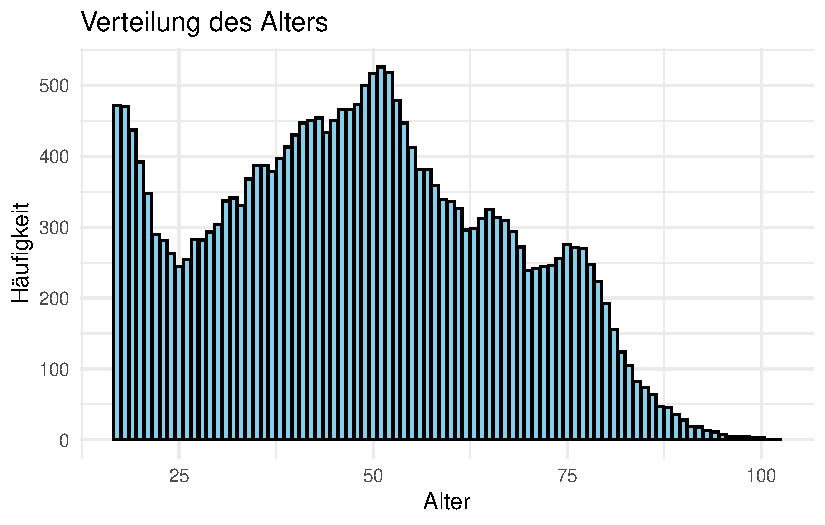
\includegraphics[keepaspectratio]{1_uebungsblatt_files/figure-pdf/unnamed-chunk-8-1.pdf}}

\subsection{Übung}\label{uxfcbung-2}

Wir alt ist die jüngste und wie alt die älteste Person?

\begin{Shaded}
\begin{Highlighting}[]
\FunctionTok{summary}\NormalTok{(df}\SpecialCharTok{$}\NormalTok{alter)}
\end{Highlighting}
\end{Shaded}

\begin{verbatim}
   Min. 1st Qu.  Median    Mean 3rd Qu.    Max. 
  17.00   34.00   48.00   48.28   62.00  102.00 
\end{verbatim}

\subsection{Übung}\label{uxfcbung-3}

Welcher Variablentyp ist Geschlecht (sex)? Welcher Alter? Welcher
Bildung?

\begin{Shaded}
\begin{Highlighting}[]
\FunctionTok{glimpse}\NormalTok{(df)}
\end{Highlighting}
\end{Shaded}

\begin{verbatim}
Rows: 23,522
Columns: 15
$ id          <int> 194, 194, 194, 194, 194, 19052, 27495, 27495, 27495, 22539~
$ syear       <int> 2015, 2016, 2017, 2018, 2019, 2015, 2016, 2018, 2019, 2015~
$ sex         <chr> "[1] weiblich", "[1] weiblich", "[1] weiblich", "[1] weibl~
$ alter       <int> 59, 60, 61, 62, 63, 74, 35, 37, 38, 85, 73, 74, 43, 44, 45~
$ anz_pers    <int> 2, 2, 2, 2, 2, 2, 3, 3, 3, 2, 1, 1, 4, 4, 4, 4, 4, 2, 2, 2~
$ anz_kind    <int> 0, 0, 0, 0, 0, 0, 1, 1, 1, 0, 0, 0, 2, 2, 2, 2, 2, 0, 0, 0~
$ bildung     <dbl> 10.5, 10.5, 10.5, 10.5, 10.5, 10.0, 15.0, 15.0, 15.0, 18.0~
$ erwerb      <chr> "[2] Teilzeitbeschäftigung", "[2] Teilzeitbeschäftigung", ~
$ branche     <chr> "[84] Oeffentliche Verwaltung, Verteidigung; Sozialversich~
$ gesund_org  <chr> "[4] Weniger gut", "[3] Zufriedenstellend", "[3] Zufrieden~
$ lebensz_org <chr> "6", "5", "7", "5", "6", "8", "8", "8", "8", "8", "5", "8"~
$ einkommenj1 <dbl> 28678.94, 19962.29, 22227.68, 22100.38, 23157.92, 0.00, 14~
$ einkommenj2 <dbl> 0.000, 0.000, 0.000, 0.000, 0.000, 0.000, 0.000, 0.000, 0.~
$ einkommenm1 <dbl> 1659.1285, 1809.3364, 1849.0375, 1616.5137, 1901.0012, 0.0~
$ einkommenm2 <dbl> 0, 0, 0, 0, 0, 0, 0, 0, 0, 0, 0, 0, 0, 0, 0, 0, 0, 0, 0, 0~
\end{verbatim}

\subsection{Übung}\label{uxfcbung-4}

Wie viele Beobachtungen gibt es pro Jahr?

\begin{Shaded}
\begin{Highlighting}[]
\FunctionTok{table}\NormalTok{(df}\SpecialCharTok{$}\NormalTok{syear)}
\end{Highlighting}
\end{Shaded}

\begin{verbatim}

2015 2016 2017 2018 2019 
5527 4987 4720 4351 3937 
\end{verbatim}

\subsection{Übung}\label{uxfcbung-5}

Was beinhaltet die Variable ``einkommenj1'' und ``einkommenj2''?

\begin{Shaded}
\begin{Highlighting}[]
\NormalTok{df\_labels}
\end{Highlighting}
\end{Shaded}

\begin{verbatim}
      variable                      variable_label
1           id Personennummer (zufällig generiert)
2        syear                       Erhebungsjahr
3          sex                          Geschlecht
4        alter          Alter der Befragungsperson
5     anz_pers         Anzahl Personen im Haushalt
6     anz_kind           Anzahl Kinder im Haushalt
7      bildung            Anzahl an Bildungsjahren
8       erwerb                       Erwerbsstatus
9      branche             Branche aktueller Beruf
10  gesund_org                    subj. Gesundheit
11 lebensz_org            Ggw. Lebenszufriedenheit
12 einkommenj1     Bruttoeinkommen/Jahr Hauptberuf
13 einkommenj2     Bruttoeinkommen/Jahr Nebenberuf
14 einkommenm1    Bruttoeinkommen/Monat Hauptberuf
15 einkommenm2    Bruttoeinkommen/Monat Nebenberuf
\end{verbatim}

\subsection{Übung}\label{uxfcbung-6}

Erstelle einen Vektor, der die Ausprägungen der Variable ``gesund\_org''
enthält. Und schaue Dir diesen Vektor an.

\begin{Shaded}
\begin{Highlighting}[]
\CommentTok{\# Eindeutige Ausprägungen der Variable \textquotesingle{}gesund\_org\textquotesingle{}}
\NormalTok{vektor\_gesund\_org }\OtherTok{\textless{}{-}} \FunctionTok{unique}\NormalTok{(df}\SpecialCharTok{$}\NormalTok{gesund\_org)}

\CommentTok{\# Ausgabe der eindeutigen Ausprägungen}
\FunctionTok{print}\NormalTok{(vektor\_gesund\_org)}
\end{Highlighting}
\end{Shaded}

\begin{verbatim}
[1] "[4] Weniger gut"       "[3] Zufriedenstellend" "[5] Schlecht"         
[4] "[2] Gut"               ""                      "[1] Sehr gut"         
\end{verbatim}

\subsection{Übung}\label{uxfcbung-7}

Wir möchten den subjektiven Gesundheitsstatus als numerische Variable
nutzen. Wir müssen daher die Variable gesund\_org in eine numerische
Variable umwandeln. Achte auf fehlende Werte.

\begin{Shaded}
\begin{Highlighting}[]
\FunctionTok{table}\NormalTok{(df}\SpecialCharTok{$}\NormalTok{gesund\_org, }\AttributeTok{useNA =} \StringTok{"always"}\NormalTok{)}
\end{Highlighting}
\end{Shaded}

\begin{verbatim}

                               [1] Sehr gut               [2] Gut 
                  102                  2535                  9488 
[3] Zufriedenstellend       [4] Weniger gut          [5] Schlecht 
                 7576                  3089                   732 
                 <NA> 
                    0 
\end{verbatim}

\begin{Shaded}
\begin{Highlighting}[]
\CommentTok{\# Ersetze leere Zeichenketten "" durch NA in der Spalte \textquotesingle{}gesund\_org\textquotesingle{}}
\NormalTok{df}\SpecialCharTok{$}\NormalTok{gesund\_org[df}\SpecialCharTok{$}\NormalTok{gesund\_org }\SpecialCharTok{==} \StringTok{""}\NormalTok{] }\OtherTok{\textless{}{-}} \ConstantTok{NA}

\CommentTok{\# Extrahiere die numerischen Werte aus der Spalte \textquotesingle{}gesund\_org\textquotesingle{}}
\NormalTok{df}\SpecialCharTok{$}\NormalTok{gesund\_org\_numeric }\OtherTok{\textless{}{-}} \FunctionTok{as.numeric}\NormalTok{(}\FunctionTok{sub}\NormalTok{(}\StringTok{"}\SpecialCharTok{\textbackslash{}\textbackslash{}}\StringTok{[([0{-}9]+)}\SpecialCharTok{\textbackslash{}\textbackslash{}}\StringTok{].*"}\NormalTok{, }\StringTok{"}\SpecialCharTok{\textbackslash{}\textbackslash{}}\StringTok{1"}\NormalTok{, df}\SpecialCharTok{$}\NormalTok{gesund\_org))}

\CommentTok{\# Überprüfe die Änderungen}
\FunctionTok{table}\NormalTok{(df}\SpecialCharTok{$}\NormalTok{gesund\_org\_numeric, }\AttributeTok{useNA =} \StringTok{"always"}\NormalTok{)}
\end{Highlighting}
\end{Shaded}

\begin{verbatim}

   1    2    3    4    5 <NA> 
2535 9488 7576 3089  732  102 
\end{verbatim}

\begin{Shaded}
\begin{Highlighting}[]
\FunctionTok{table}\NormalTok{(df}\SpecialCharTok{$}\NormalTok{gesund\_org, }\AttributeTok{useNA =} \StringTok{"always"}\NormalTok{)}
\end{Highlighting}
\end{Shaded}

\begin{verbatim}

         [1] Sehr gut               [2] Gut [3] Zufriedenstellend 
                 2535                  9488                  7576 
      [4] Weniger gut          [5] Schlecht                  <NA> 
                 3089                   732                   102 
\end{verbatim}

\subsection{Übung}\label{uxfcbung-8}

Stelle die Verteilung des subjetiven Gesundheitsstatus graphisch dar

\begin{Shaded}
\begin{Highlighting}[]
\CommentTok{\# Barplot erstellen}
\FunctionTok{ggplot}\NormalTok{(df, }\FunctionTok{aes}\NormalTok{(}\AttributeTok{x =} \FunctionTok{factor}\NormalTok{(gesund\_org\_numeric))) }\SpecialCharTok{+}
  \FunctionTok{geom\_bar}\NormalTok{(}\AttributeTok{fill =} \StringTok{"skyblue"}\NormalTok{, }\AttributeTok{color =} \StringTok{"black"}\NormalTok{) }\SpecialCharTok{+}
  \FunctionTok{labs}\NormalTok{(}
    \AttributeTok{title =} \StringTok{"Univariate Verteilung des subjektiven Gesundheitsstatus"}\NormalTok{,}
    \AttributeTok{x =} \StringTok{"Subjektiver Gesundheitsstatus (1 = Sehr gut, 5 = Schlecht)"}\NormalTok{,}
    \AttributeTok{y =} \StringTok{"Häufigkeit"}
\NormalTok{  ) }\SpecialCharTok{+}
  \FunctionTok{theme\_minimal}\NormalTok{()}
\end{Highlighting}
\end{Shaded}

\pandocbounded{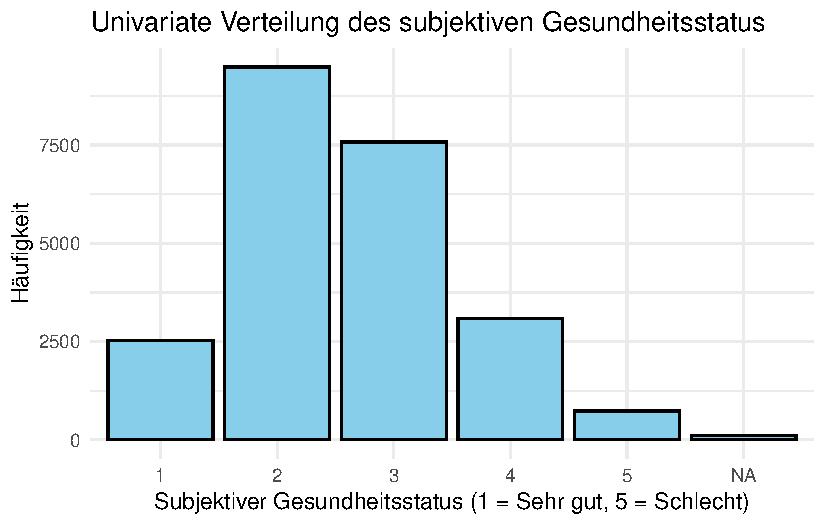
\includegraphics[keepaspectratio]{1_uebungsblatt_files/figure-pdf/unnamed-chunk-15-1.pdf}}

\subsection{Übung}\label{uxfcbung-9}

Gibt es fehlende Werte auf der Variable monatliches Einkommen
(einkommenm1) und auf der Variable Alter?

\begin{Shaded}
\begin{Highlighting}[]
\FunctionTok{table}\NormalTok{(df}\SpecialCharTok{$}\NormalTok{alter, }\AttributeTok{useNA =} \StringTok{"always"}\NormalTok{)}
\end{Highlighting}
\end{Shaded}

\begin{verbatim}

  17   18   19   20   21   22   23   24   25   26   27   28   29   30   31   32 
 472  470  437  392  347  290  281  263  244  254  283  282  293  304  337  341 
  33   34   35   36   37   38   39   40   41   42   43   44   45   46   47   48 
 331  368  387  387  379  397  413  430  447  450  454  434  450  466  466  473 
  49   50   51   52   53   54   55   56   57   58   59   60   61   62   63   64 
 500  517  526  518  479  447  412  381  381  359  339  336  326  296  298  312 
  65   66   67   68   69   70   71   72   73   74   75   76   77   78   79   80 
 325  314  309  294  272  239  242  244  246  256  276  271  270  247  223  192 
  81   82   83   84   85   86   87   88   89   90   91   92   93   94   95   96 
 156  124  105   82   74   64   47   46   36   28   19   18   13   11    8    5 
  97   98   99  100  101  102 <NA> 
   5    4    3    3    1    1    0 
\end{verbatim}

\begin{Shaded}
\begin{Highlighting}[]
\FunctionTok{summary}\NormalTok{(df}\SpecialCharTok{$}\NormalTok{einkommenm1)}
\end{Highlighting}
\end{Shaded}

\begin{verbatim}
   Min. 1st Qu.  Median    Mean 3rd Qu.    Max. 
    0.0     0.0   852.9  1645.6  2687.4 35260.9 
\end{verbatim}

\subsection{Übung}\label{uxfcbung-10}

Schaue Dir den Zusammenhang von subjektiven Gesundheitsstatus und Alter
graphisch mit Hilfe eines Scatterplots an. Beschränke die Daten auf das
Jahr 2019 und auf Personen, die jünger als 65 Jahre alt sind.

\begin{Shaded}
\begin{Highlighting}[]
\CommentTok{\# Scatterplot mit ggplot2 erstellen}
\FunctionTok{ggplot}\NormalTok{(df }\SpecialCharTok{\%\textgreater{}\%} \FunctionTok{filter}\NormalTok{(syear}\SpecialCharTok{==}\StringTok{"2019"}\NormalTok{, alter }\SpecialCharTok{\textless{}} \DecValTok{65}\NormalTok{), }\FunctionTok{aes}\NormalTok{(}\AttributeTok{x =}\NormalTok{ alter , }\AttributeTok{y =}\NormalTok{ einkommenm1)) }\SpecialCharTok{+}
  \FunctionTok{geom\_point}\NormalTok{(}\AttributeTok{color =} \StringTok{"blue"}\NormalTok{, }\AttributeTok{alpha =} \FloatTok{0.6}\NormalTok{) }\SpecialCharTok{+}  \CommentTok{\# Punkte hinzufügen}
  \FunctionTok{geom\_smooth}\NormalTok{(}\AttributeTok{method =} \StringTok{"lm"}\NormalTok{, }\AttributeTok{color =} \StringTok{"red"}\NormalTok{, }\AttributeTok{se =} \ConstantTok{TRUE}\NormalTok{) }\SpecialCharTok{+}  \CommentTok{\# Lineare Trendlinie mit Konfidenzintervall}
  \FunctionTok{labs}\NormalTok{(}
    \AttributeTok{title =} \StringTok{"Zusammenhang zwischen Einkommen und Alter"}\NormalTok{,}
    \AttributeTok{x =} \StringTok{"Alter"}\NormalTok{,}
    \AttributeTok{y =} \StringTok{"Einkommen"}
\NormalTok{  ) }\SpecialCharTok{+}
  \FunctionTok{theme\_minimal}\NormalTok{()  }\CommentTok{\# Minimalistisches Theme}
\end{Highlighting}
\end{Shaded}

\begin{verbatim}
`geom_smooth()` using formula = 'y ~ x'
\end{verbatim}

\pandocbounded{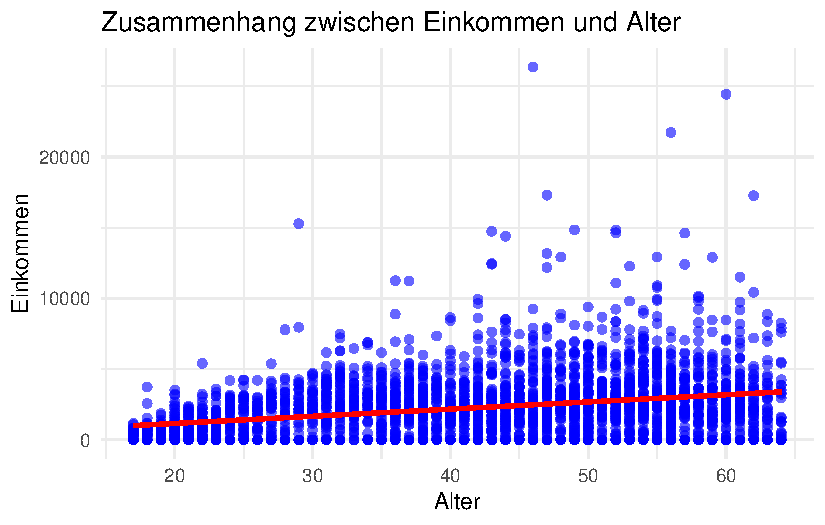
\includegraphics[keepaspectratio]{1_uebungsblatt_files/figure-pdf/unnamed-chunk-17-1.pdf}}

\subsection{Übung}\label{uxfcbung-11}

Und nun mit logarithmiertem Einkommen. Was fällt auf?

\begin{Shaded}
\begin{Highlighting}[]
\CommentTok{\# Scatterplot mit ggplot2 erstellen}
\FunctionTok{ggplot}\NormalTok{(df }\SpecialCharTok{\%\textgreater{}\%} \FunctionTok{filter}\NormalTok{(syear}\SpecialCharTok{==}\StringTok{"2019"}\NormalTok{, alter }\SpecialCharTok{\textless{}} \DecValTok{65}\NormalTok{), }\FunctionTok{aes}\NormalTok{(}\AttributeTok{x =}\NormalTok{ alter , }\AttributeTok{y =} \FunctionTok{log}\NormalTok{(einkommenm1))) }\SpecialCharTok{+}
  \FunctionTok{geom\_point}\NormalTok{(}\AttributeTok{color =} \StringTok{"blue"}\NormalTok{, }\AttributeTok{alpha =} \FloatTok{0.6}\NormalTok{) }\SpecialCharTok{+}  \CommentTok{\# Punkte hinzufügen}
  \FunctionTok{geom\_smooth}\NormalTok{(}\AttributeTok{method =} \StringTok{"lm"}\NormalTok{, }\AttributeTok{color =} \StringTok{"red"}\NormalTok{, }\AttributeTok{se =} \ConstantTok{TRUE}\NormalTok{) }\SpecialCharTok{+}  \CommentTok{\# Lineare Trendlinie mit Konfidenzintervall}
  \FunctionTok{labs}\NormalTok{(}
    \AttributeTok{title =} \StringTok{"Zusammenhang zwischen Einkommen und Alter"}\NormalTok{,}
    \AttributeTok{x =} \StringTok{"Alter"}\NormalTok{,}
    \AttributeTok{y =} \StringTok{"Einkommen, log."}
\NormalTok{  ) }\SpecialCharTok{+}
  \FunctionTok{theme\_minimal}\NormalTok{()  }\CommentTok{\# Minimalistisches Theme}
\end{Highlighting}
\end{Shaded}

\begin{verbatim}
`geom_smooth()` using formula = 'y ~ x'
\end{verbatim}

\begin{verbatim}
Warning: Removed 660 rows containing non-finite outside the scale range
(`stat_smooth()`).
\end{verbatim}

\pandocbounded{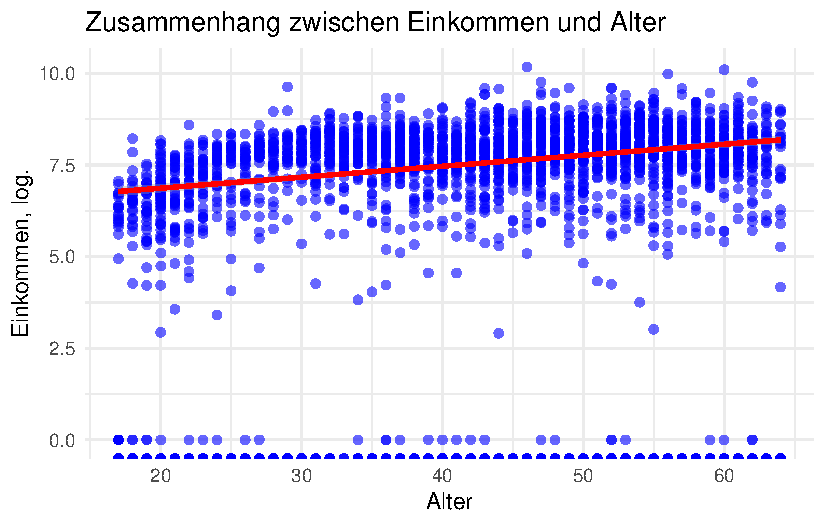
\includegraphics[keepaspectratio]{1_uebungsblatt_files/figure-pdf/unnamed-chunk-18-1.pdf}}

\subsection{Übung}\label{uxfcbung-12}

Wandle dieses Dokument in ein PDF und ein HTML Dokument um.

\section{Weiterführende Literatur}\label{weiterfuxfchrende-literatur}

\begin{itemize}
\tightlist
\item
  \href{https://r4ds.had.co.nz/}{R for Data Science}
\end{itemize}




\end{document}
